\documentclass[11pt]{article}
%Gummi|065|=)
\title{\textbf{CV Homework 2}}
\author{Eric Feuvrier Danziger\\
		}
\date{}
\usepackage{graphicx}
\usepackage{float}
\begin{document}

\maketitle




\section*{2.4.1 Testing and Choosing Ratio}
I designed the test based on the idea of second nearest neighbor explained in the paper. The idea is to use Hamming distance, where the measure of distance is the number of digits that are different. There are of course always an array of closest points, but if the difference between the distance to the first closest and second closest is great, it suggests that the first closest is much better than the second closest. Alternatively, if the second closest is similar in distance to the first closest, it is likely that neither is a match to the point. To be a match to a point, you have to be much closer than the rest of the pack. 

I chose a ratio of 0.7 because it gave me many points without any (at least on the image pair I tested) errors. I wanted a high enough value to ensure many points to allow for the best comparison of objects, without misplaced points. The paper recommended 0.8, but this still had a few points that were not good matches. 
\begin{figure}[H]
\centering
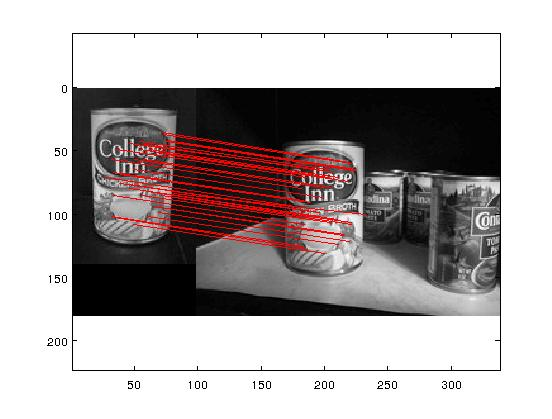
\includegraphics[width=90mm]{ratiopoint7.jpg}
\caption{Matched with 0.7 ratio}
\end{figure}

\begin{figure}[H]
\centering
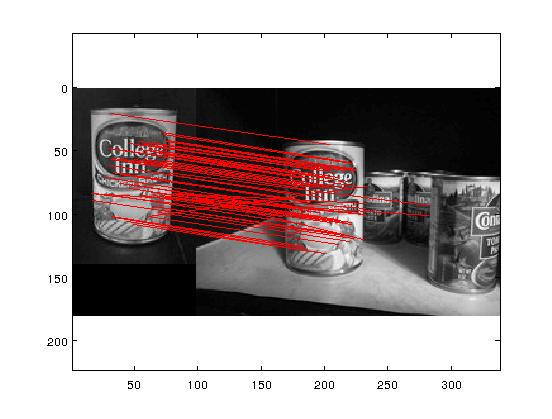
\includegraphics[width=90mm]{ratiopoint8.jpg}
\caption{Matched with 0.8 ratio - there are some mismatches}
\end{figure}

\begin{figure}[H]
\centering
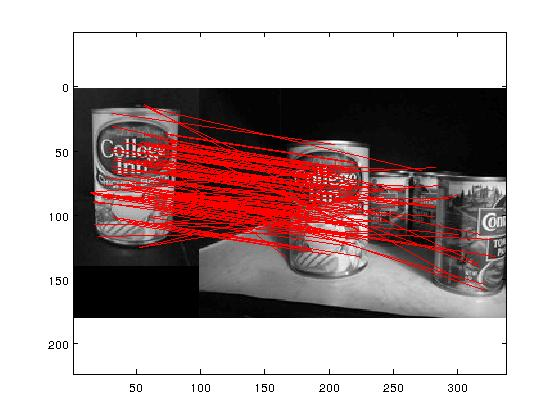
\includegraphics[width=90mm]{ratiopoint9.jpg}
\caption{Matched with 0.9 ratio - more mismatches}
\end{figure}

\section*{2.4.2 Image Matches}
This is an example of a match of chickenbroth images.
\begin{figure}[H]
\centering
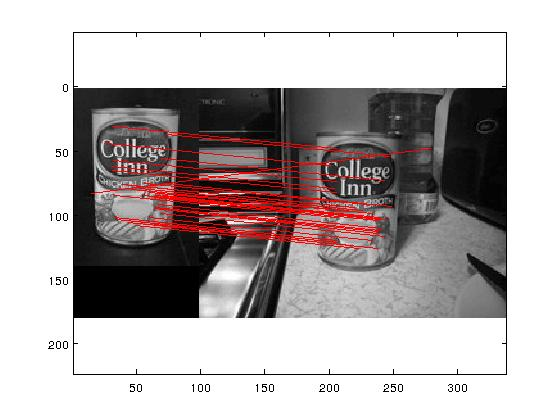
\includegraphics[width=90mm]{model_to_3.jpg}
\caption{Model and image 03 matched with 0.7 ratio}
\end{figure}

The Taj images:
\begin{figure}[H]
\centering
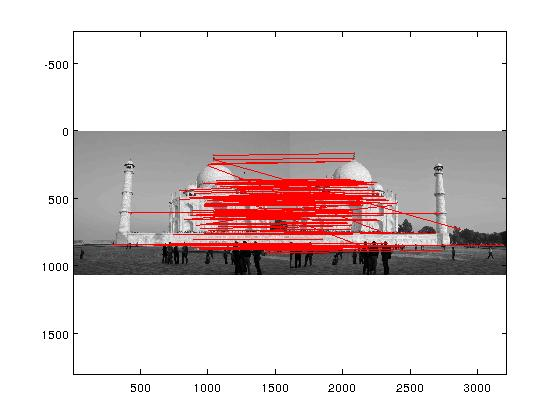
\includegraphics[width=90mm]{taj.jpg}
\caption{Taj matched with 0.7 ratio \label{taj}}
\end{figure}

Some textbook images:
\begin{figure}[H]
\centering
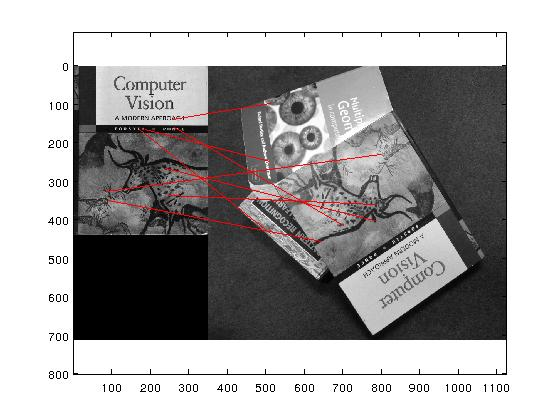
\includegraphics[width=90mm]{pile.jpg}
\caption{Pile matched with 0.7 ratio }
\end{figure}

\begin{figure}[H]
\centering
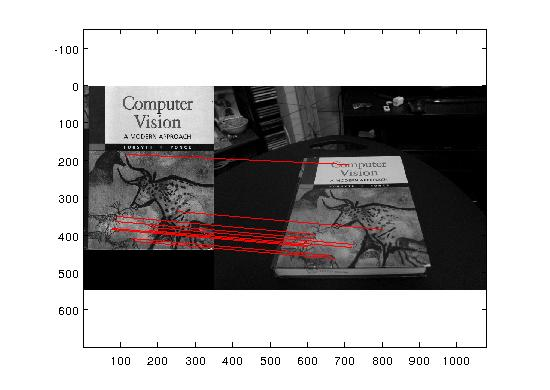
\includegraphics[width=90mm]{desk.jpg}
\caption{Desk matched with 0.7 ratio }
\end{figure}

\begin{figure}[H]
\centering
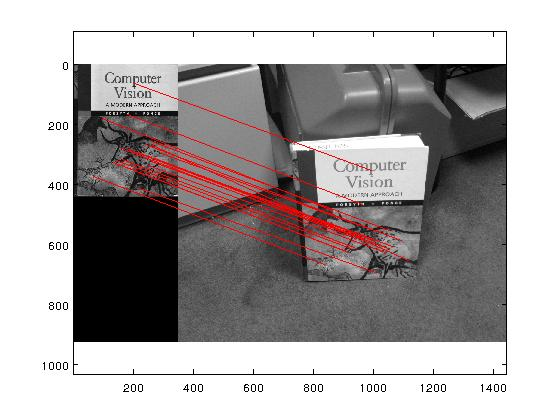
\includegraphics[width=90mm]{stand.jpg}
\caption{Stand matched with 0.7 ratio }
\end{figure}

\begin{figure}[H]
\centering
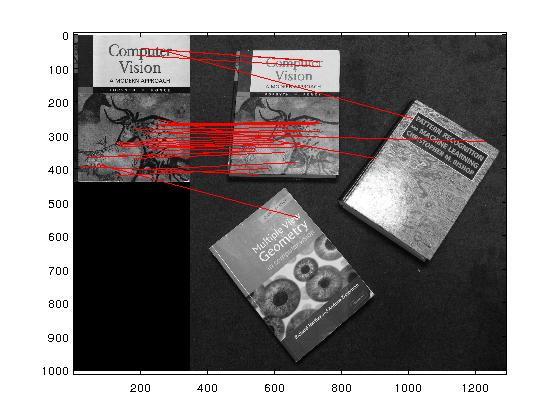
\includegraphics[width=90mm]{floor.jpg}
\caption{Floor matched with 0.7 ratio }
\end{figure}

\begin{figure}[H]
\centering
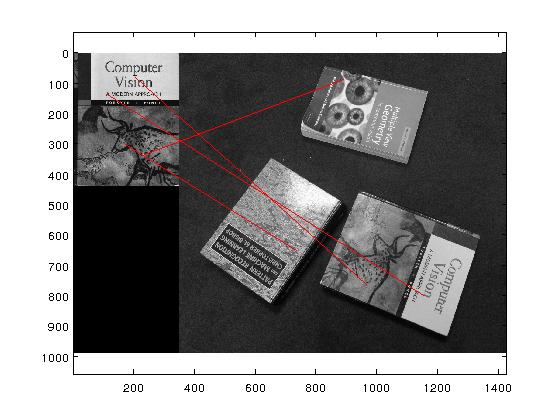
\includegraphics[width=90mm]{floor_rotated.jpg}
\caption{Floor Rotated matched with 0.7 ratio }
\end{figure}

As you can see, rotated images perform worse. There are less matches, because the descriptors have more problems lining up since there is no way to account for rotation of an interest point. Different perspectives (desk and stand) have more matching points than rotated ones. 

This makes sense when you consider how the BRIEF descriptor works, treating each patch as upright with respect to the image coordinate frame. 

\section*{Rotation}
\begin{figure}[H]
\centering
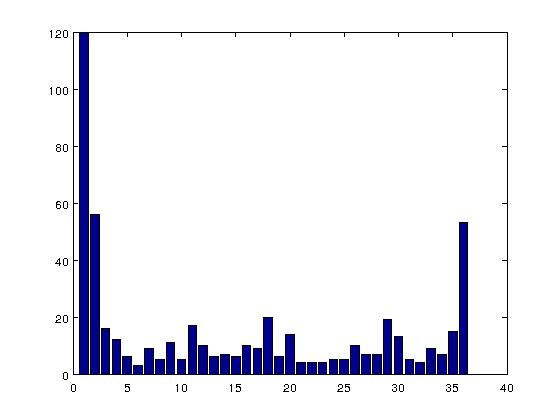
\includegraphics[width=90mm]{rotation_bar_chart.jpg}
\caption{Matches per 10 degrees rotation}
\end{figure}

You can see the unrotated image is by far the best, with the least amount of rotation coming in second (the second value and last value, each with 10 degrees rotation). The rest of the rotated values are bad, with some random noise creating differences in values. This is because of the way the BRIEF descriptor creates descriptions of patches. 


\end{document}
